\chapter{Goal, domain of application and responsibilities}

\section{Introduction}

The \telemacsystem{} is an integrated suite of solvers for use in the field of
free-surface flow. Having been used in the context of many studies throughout
the world, it has become one of the major standards in its field.
The \telemacsystem{} is managed by a Consortium of core organisations: Artelia
(France), BundesAnstalt für Wasserbau (BAW, Germany), Centre d’Études et
d'expertise sur les Risques, l'Environnement, la Mobilité et l'Aménagement
(CEREMA, France), Centre Européen de Recherche et de Formation Avancée en
Calcul Scientifique (CERFACS, France), Daresbury Laboratory (United Kingdom),
Électricité de France R\&D (EDF, France), HR Wallingford (United Kingdom),
International Marine and Dredging Consultants (IMDC, Belgium) and École des
Ponts ParisTech (France).\\

The \telemacsystem{} is used by most partners for dimensioning and impact
studies, where safety is prevailing and, for this reason, reliability,
validation and a worldwide recognition of our tools are of utmost importance.
As a consequence and to improve access to the \telemacsystem{} for the whole
community of consultants and researchers, the choice of the open source has
been made. Anyone can thus take advantage of the \telemacsystem{} and assess
its performances.\\

This Quality Plan describes the general dispositions in place to ensure the
quality of the \telemacsystem{} and its services.

\section{Description of the software}

The \telemacsystem{} is composed of several modules including numerical models
and resolution algorithms useful for its utilisation.\\

The \telemacsystem{} and its tools are open source, under GPL license, with the
\bief{} finite element library under LGPL\@. It is available from the
\telemacsystem{} website (\url{www.opentelemac.org}). This website is the main
access to the \telemacsystem{} information and documentation.\\

The \telemacsystem{} can use external software and libraries. This Quality Plan
does not cover those external elements (MPI, METIS, MED\ldots), it only covers
the functions using them in the code.\\

This quality plan should guarantee the interoperability between the
\telemacsystem{} modules and software used for pre- and post-processing (such
as Fudaa, Salome\ldots).  The minimum requirements for interoperability are
to follow the same standard as any development in the \telemacsystem{}
(Chapter~\ref{devplan}).

\begin{figure}[H]
  \centering
  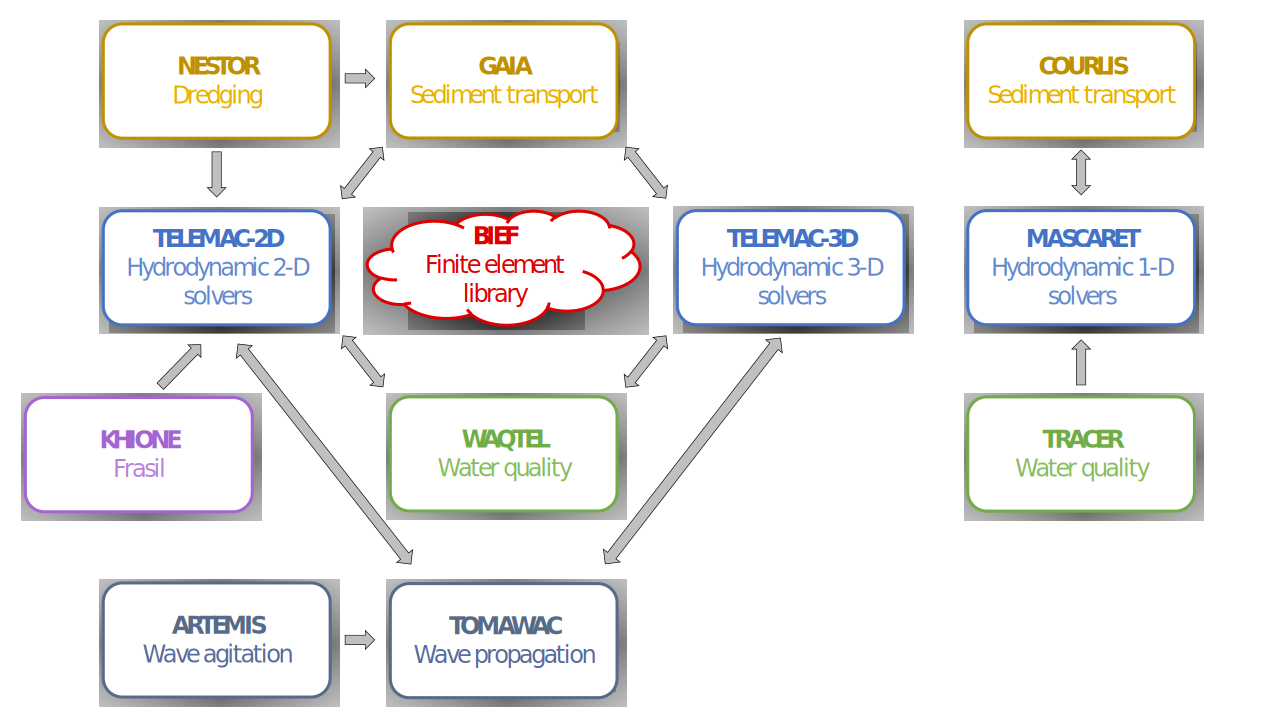
\includegraphics[scale=0.4]{graphics/telemac-modules.png}
\caption{\label{telma_codes} Modules of the \telemacsystem{}}
\end{figure}

\section{Versions concerned}

This Software Quality Plan (SQP) is applied since version 7.0 of \tel{} and
version 8.0 of \mascaret.

\section{Quality Plan Maintainers}

The purpose of this paragraph is to identify the people in charge of the
creation, verification, validation and follow-up of the Software Quality Plan.
The document 'Organisation of the \telemacsystem{} activity' in
Appendix~\ref{fullorga} gives more details on the organisation and on the
action in their charge. The Appendix~\ref{peopleoftelma} gives a nominative
list for those roles.

\subsection{Quality Handler}

The Quality Handler (QH) is the \telemacsystem{} Project Manager (PM). He is in
charge of the creation and the follow-up of the Software Quality Plan. He can
be helped by the Code Handlers (CH) to whom he can delegate the implementation
of the necessary changes. He has to verify that the applied action complies
with the SQP\@.

\section{Evolution of the Software Quality Plan}

The evolution of the Software Quality Plan and its complementary documents can
result from the following actions:
\begin{itemize}
\item Evolution of the Quality procedure in EDF R\&D.
\item Evolution of the organisation inside the Consortium.
\item Evolution of the handling procedure for the software.
\item An extension of the applicable domain.
\end{itemize}

\section{Case of non application of the Software Quality Plan}

In case the SQP or part of it cannot be applied, a derogation is possible, if
validated by the QH\@. This derogation is traced in a document with the Software
Quality Plan. Otherwise a modification of the SQP can be asked by the QH so
the SQP could be applicable again.
